
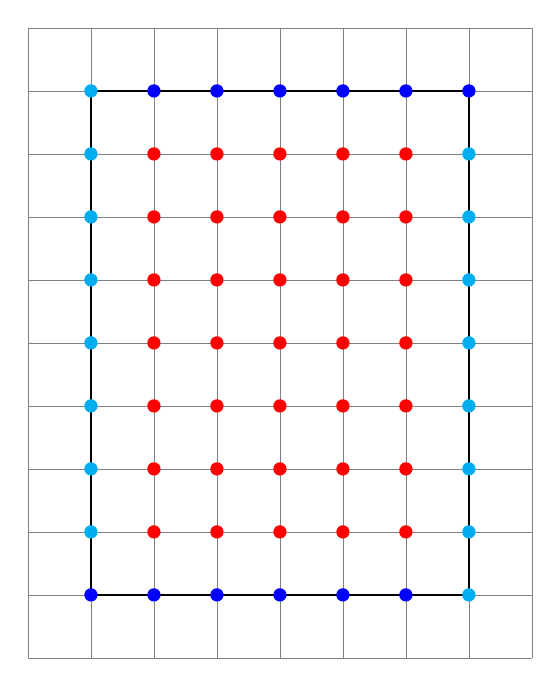
\begin{tikzpicture}[scale=.8]
  \draw[gray, very thin] (0,0) grid (8,10);
  \draw[thick] (1,1) rectangle (7,9);
  \foreach \x in {2,...,6} {
    \foreach \y in {2,...,8} { \fill[red] (\x,\y) circle (3pt); }
  }
  \foreach \x in {1,...,6} {
    \fill[blue] (\x,1) circle (3pt) (\x+1,9) circle (3pt); }
  \foreach \y in {2,...,9} {
    \fill[cyan] (1,\y) circle (3pt) (7,\y-1) circle (3pt); }
\end{tikzpicture}
